\documentclass[11pt,a4paper]{article}

% ─── Packages ────────────────────────────────────────────────────────────────
\usepackage[margin=2.2cm]{geometry}
\usepackage{microtype}
\usepackage{amsmath,amssymb,mathtools}
\usepackage{booktabs}
\usepackage{array}
\usepackage{graphicx}
\usepackage{xcolor}
\usepackage{hyperref}
\usepackage{enumitem}
\usepackage{float}
\usepackage{fancyhdr}
\usepackage{tikz}
\usetikzlibrary{arrows.meta,positioning,shapes.geometric,calc}

\hypersetup{
  colorlinks=true,
  linkcolor=blue!60!black,
  citecolor=green!50!black,
  urlcolor=blue!70!black
}

\pagestyle{fancy}
\fancyhf{}
\fancyhead[L]{\small LHCb Track Extrapolation}
\fancyhead[R]{\small \thepage}
\renewcommand{\headrulewidth}{0.4pt}

\newcommand{\dz}{\Delta z}
\newcommand{\qop}{q/p}
\newcommand{\bvec}[1]{\mathbf{#1}}
\newcommand{\vstate}{\bvec{s}}
\newcommand{\clgt}{c_\text{light}}

\title{%
  \textbf{Runge--Kutta Track Extrapolation in the LHCb Software Stack}\\[6pt]
  \large Mathematical Foundations, Numerical Schemes, and the QMTest Workflow
}
\author{Auto-generated Technical Reference}
\date{March 2026}

\begin{document}
\maketitle
\tableofcontents
\newpage

%=============================================================================
\section{Introduction}
%=============================================================================

Track extrapolation is the process of propagating a charged particle's state
through the LHCb detector from one $z$-plane to another, accounting for the
deflection due to the dipole magnetic field and (optionally) energy loss and
multiple scattering in detector material. The extrapolation engine solves the
equations of motion for a charged particle in a magnetic field numerically,
using several Runge--Kutta (RK) variants.

This document provides:
\begin{enumerate}[leftmargin=2em]
  \item The equations of motion being solved (Section~\ref{sec:eom}).
  \item The state vector and transport matrix conventions (Section~\ref{sec:statevec}).
  \item Mathematical derivations for every RK scheme implemented:
    Cash--Karp, Dormand--Prince, Bogacki--Shampine, Verner, STEP/RKN, Herab,
    Kisel, and the parabolic single-step approximation (Sections~\ref{sec:rk}--\ref{sec:parabolic}).
  \item The adaptive step-size control algorithm (Section~\ref{sec:stepsize}).
  \item The analytic Jacobian propagation (Section~\ref{sec:jacobian}).
  \item The \texttt{TrackMasterExtrapolator} dispatch logic (Section~\ref{sec:master}).
  \item The QMTest regression testing pipeline (Section~\ref{sec:qmtest}).
\end{enumerate}


%=============================================================================
\section{State Vector and Conventions}\label{sec:statevec}
%=============================================================================

All LHCb extrapolators represent the track state at a given $z$-position as a
five-component vector:
\begin{equation}\label{eq:statevec}
  \vstate = \begin{pmatrix} x \\ y \\ t_x \\ t_y \\ \qop \end{pmatrix}
  \quad\text{at position } z,
\end{equation}
where $x,y$ are the transverse positions, $t_x = dx/dz$ and $t_y = dy/dz$ are
the direction tangents, and $\qop$ is the charge divided by the total momentum.
The independent variable is $z$ (the beam axis), not time.

The \textbf{transport matrix} (Jacobian) is a $5\times5$ matrix $F$ satisfying
\begin{equation}
  \vstate_\text{out} \approx F \cdot \vstate_\text{in},
\end{equation}
used to propagate the covariance matrix via the similarity transformation
\begin{equation}
  C_\text{out} = F \, C_\text{in} \, F^T.
\end{equation}


%=============================================================================
\section{Equations of Motion}\label{sec:eom}
%=============================================================================

A charged particle with charge $q$ and momentum $p$ in a magnetic field
$\bvec{B} = (B_x, B_y, B_z)$ obeys the Lorentz force law. In the
$(x,y,t_x,t_y)$ representation with $z$ as the independent variable, the
ODE is:
\begin{equation}\label{eq:eom}
  \frac{d}{dz}
  \begin{pmatrix} x \\ y \\ t_x \\ t_y \end{pmatrix}
  =
  \begin{pmatrix} t_x \\ t_y \\ (\qop)\,\clgt\, \mathcal{A}_x \\ (\qop)\,\clgt\, \mathcal{A}_y \end{pmatrix},
\end{equation}
where
\begin{equation}
  n = \sqrt{1 + t_x^2 + t_y^2},
\end{equation}
\begin{align}
  \mathcal{A}_x &= n\bigl[\,t_y(t_x B_x + B_z) - (1+t_x^2)\,B_y\,\bigr], \label{eq:Ax} \\[4pt]
  \mathcal{A}_y &= n\bigl[\,-t_x(t_y B_y + B_z) + (1+t_y^2)\,B_x\,\bigr], \label{eq:Ay}
\end{align}
and $\clgt = 299.792458~\text{mm/ns}$ converts from natural units (Gaudi convention).

\paragraph{Physical justification.}
The terms $\mathcal{A}_x$ and $\mathcal{A}_y$ arise from projecting the
three-dimensional Lorentz force $\bvec{F} = q\,\bvec{v}\times\bvec{B}$ onto
the $(x,y)$ plane using the chain rule $dt_x/dz = (dt_x/dt)(dt/dz)$. The
factor $n$ accounts for the arc-length correction $ds/dz = n$, and the $q/p$
factor appears because the Lorentz force changes direction but not speed,
giving the curvature $\kappa \propto q B / p$.


%=============================================================================
\section{General Adaptive Runge--Kutta Framework}\label{sec:rk}
%=============================================================================

\subsection{Embedded RK Pairs}

An \textit{embedded} Runge--Kutta method of order $p(p-1)$ computes two
estimates of the solution at each step: a higher-order estimate $\bvec{y}_{n+1}$
used to advance the solution, and a lower-order estimate
$\hat{\bvec{y}}_{n+1}$ used solely for error control. The method is defined by
its \textbf{Butcher tableau}:
\begin{equation}
  \renewcommand{\arraystretch}{1.3}
  \begin{array}{c|cccc}
    c_1    & & & & \\
    c_2    & a_{21} & & & \\
    \vdots & \vdots & \ddots & & \\
    c_s    & a_{s1} & \cdots & a_{s,s-1} & \\
    \hline
           & b_1 & b_2 & \cdots & b_s \\
           & b^*_1 & b^*_2 & \cdots & b^*_s
  \end{array}
\end{equation}

The stage values are computed as:
\begin{equation}\label{eq:rk-stages}
  \bvec{k}_i = h\,\bvec{f}\!\left(z_n + c_i h,\;\bvec{y}_n + \sum_{j=1}^{i-1} a_{ij}\,\bvec{k}_j\right),
  \qquad i = 1,\ldots,s,
\end{equation}
and the two estimates are:
\begin{align}
  \bvec{y}_{n+1} &= \bvec{y}_n + \sum_{i=1}^{s} b_i\,\bvec{k}_i \quad\text{(order $p$)}, \label{eq:rk-update}\\
  \hat{\bvec{y}}_{n+1} &= \bvec{y}_n + \sum_{i=1}^{s} b^*_i\,\bvec{k}_i \quad\text{(order $p-1$)}.
\end{align}
The local truncation error estimate is:
\begin{equation}\label{eq:rk-error}
  \bvec{e} = \bvec{y}_{n+1} - \hat{\bvec{y}}_{n+1} = \sum_{i=1}^{s}(b_i - b^*_i)\,\bvec{k}_i.
\end{equation}

\subsection{FSAL Property}

Some schemes (Dormand--Prince, Tsitouras) satisfy the \textit{First Same As Last}
(FSAL) property: the last stage $\bvec{k}_s$ of step $n$ equals the first
stage $\bvec{k}_1$ of step $n+1$. This saves one function evaluation per
accepted step.


%=============================================================================
\section{Cash--Karp Method (Default)}\label{sec:cashkarp}
%=============================================================================

The Cash--Karp method is a 6-stage, 5th-order embedded pair with a 4th-order
error estimator. It is the default scheme in \texttt{TrackRungeKuttaExtrapolator}.

\subsection{Butcher Tableau}

\begin{equation}
\renewcommand{\arraystretch}{1.3}
{\small
\begin{array}{c|cccccc}
  0      &         &          &             &              &           \\
  \frac{1}{5}    & \frac{1}{5}     &          &             &              &           \\
  \frac{3}{10}   & \frac{3}{40}    & \frac{9}{40}     &             &              &           \\
  \frac{3}{5}    & \frac{3}{10}    & \!-\frac{9}{10}    & \frac{6}{5}         &              &           \\
  1      & \!-\frac{11}{54}  & \frac{5}{2}      & \!-\frac{70}{27}      & \frac{35}{27}        &           \\
  \frac{7}{8}    & \frac{1631}{55296} & \frac{175}{512} & \frac{575}{13824} & \frac{44275}{110592} & \frac{253}{4096} \\[4pt]
  \hline
  b_i    & \frac{37}{378} & 0 & \frac{250}{621} & \frac{125}{594} & 0 & \frac{512}{1771} \\[4pt]
  b^*_i  & \frac{2825}{27648} & 0 & \frac{18575}{48384} & \frac{13525}{55296} & \frac{277}{14336} & \frac{1}{4}
\end{array}
}
\end{equation}

\subsection{Justification}

Cash and Karp (1990) designed this pair to minimize the leading-order
truncation error coefficient of the 5th-order formula while simultaneously
providing an efficient 4th-order embedded estimator. The choice of $c_6=7/8$
(rather than 1) places the final stage evaluation interior to the step,
providing better error estimation for stiff-like problems. Compared to the
Fehlberg~4(5) pair, Cash--Karp gives more reliable step-size estimates and is
preferred for non-stiff systems such as charged-particle tracking.


%=============================================================================
\section{Other Embedded RK Schemes}\label{sec:other-rk}
%=============================================================================

The \texttt{TrackRungeKuttaExtrapolator} supports 15 additional schemes:

\begin{table}[H]
\centering
\caption{Available embedded RK schemes in the LHCb extrapolator.}
\label{tab:schemes}
\begin{tabular}{@{}lcccl@{}}
\toprule
\textbf{Scheme} & \textbf{Stages} & \textbf{Order} & \textbf{FSAL} & \textbf{Reference} \\
\midrule
Cash--Karp (default) & 6 & 5(4) & No & Cash \& Karp, 1990 \\
Fehlberg             & 6 & 5(4) & No & Fehlberg, 1969 \\
Dormand--Prince      & 7 & 5(4) & Yes & Dormand \& Prince, 1980 \\
Bogacki--Shampine~3  & 4 & 3(2) & No & Bogacki \& Shampine, 1989 \\
Bogacki--Shampine~5  & 8 & 5(4) & No & Bogacki \& Shampine \\
Heun--Euler          & 2 & 2(1) & No & Classical \\
Sharp--Smart~5       & 7 & 5(4) & No & Sharp \& Smart \\
Tsitouras~5          & 7 & 5(4) & Yes & Tsitouras, TEI Chalkis \\
Tsitouras~2009       & 7 & 5(4) & No & AIP Conf.\ Proc.\ 1168 \\
Sharp--Verner~6      & 9 & 6(5) & Yes & SIAM J.\ Numer.\ Anal.\ 31 \\
Sharp--Verner~7      & 12& 7(6) & Yes & SIAM J.\ Numer.\ Anal.\ 31 \\
Verner~6             & 8 & 6(5) & No & Verner \\
Verner~7             & 10& 7(6) & No & Verner \\
Verner~8             & 13& 8(7) & No & Verner \\
Verner~9             & 16& 9(8) & No & Verner \\
\bottomrule
\end{tabular}
\end{table}

\subsection{Dormand--Prince 5(4)}

This is the most widely used adaptive RK scheme (MATLAB's \texttt{ode45}).
It satisfies FSAL, requiring only 6 function evaluations per accepted step.
The Butcher coefficients are optimised to minimise the local truncation error
norm:
\[
  c = \left(0,\;\tfrac{1}{5},\;\tfrac{3}{10},\;\tfrac{4}{5},\;\tfrac{8}{9},\;1,\;1\right).
\]

\subsection{Bogacki--Shampine 3(2)}

A low-order ($p=3$) pair with only 4~stages, useful when very high accuracy is
not needed but computational cost must be minimised. Each step requires only
3~function evaluations (with FSAL). It is used in the LHCb test suite for
cross-validation.

\subsection{Verner Family (6th--9th Order)}

Higher-order methods by Jim Verner provide greater accuracy per step at
the cost of more stages. The 8th-order Verner scheme with 13~stages can
take much larger steps for the same tolerance, which can be advantageous
for long propagations through weak-field regions.


%=============================================================================
\section{Adaptive Step-Size Control}\label{sec:stepsize}
%=============================================================================

Given the error estimate $\bvec{e}$ from~\eqref{eq:rk-error}, the step is
accepted or rejected based on the normalised error:

\begin{equation}
  E = \max\!\left(
    \frac{|e_x|}{\epsilon_x},\;
    \frac{|e_y|}{\epsilon_y},\;
    \frac{|e_{t_x}|}{\epsilon_{t_x} + |\Delta t_x|\,\epsilon_\text{rel}}
  \right),
\end{equation}
where $\epsilon_x = \epsilon_y = $ \texttt{Tolerance} (default $0.001$~mm)
and $\epsilon_\text{rel} = $ \texttt{RelToleranceTx} (default $5\times10^{-5}$).
The mixed absolute--relative criterion for $t_x$ prevents overly small steps
when the curvature (hence $\Delta t_x$) is large.

\subsection{Acceptance Criterion}

The step is \textbf{accepted} if $E \leq \sigma$ (default $\sigma=5.5$) or if
the step is already at the minimum step size $h_\text{min}$ (default 10~mm).
The generous threshold $\sigma > 1$ prioritises speed over strict accuracy,
relying on error cancellation across multiple steps.

\subsection{Step Scaling}

The new step size is computed via the standard PI controller:
\begin{equation}
  h_{n+1} = h_n \cdot \text{clamp}\!\left(f,\; f_\text{min},\; f_\text{max}\right),
  \qquad
  f = \begin{cases}
    \max\!\bigl(f_\text{min},\; S \cdot E^{-1/4}\bigr) & \text{if } E > 1 \;\text{(shrink)}, \\[3pt]
    \min\!\bigl(f_\text{max},\; S \cdot E^{-1/5}\bigr) & \text{if } 0 < E \leq 1 \;\text{(grow)}, \\[3pt]
    f_\text{max} & \text{if } E = 0,
  \end{cases}
\end{equation}
with safety factor $S=1.0$, $f_\text{min}=0.125$, $f_\text{max}=4.0$.

\paragraph{Mathematical basis.} For a method of order $p$, the local error
scales as $\mathcal{O}(h^{p+1})$, so to achieve a target error $\epsilon$
from a current error $E\epsilon$, the optimal scaling is
$h_\text{new}/h_\text{old} = (1/E)^{1/(p+1)}$. The shrink exponent $-1/4$
and grow exponent $-1/5$ correspond to the 4th- and 5th-order error estimates
respectively, following the prescription of Numerical Recipes.

\subsection{Termination Conditions}

The propagation terminates with failure if any of these hold:
\begin{itemize}[nosep]
  \item Curling: $\max(|t_x|, |t_y|) > 10$ (\texttt{MaxSlope}).
  \item Excessive curvature: $|(\qop)\,B_y| > 1/\text{m}$ (\texttt{MaxCurvature}).
  \item Step count: steps $\geq 1000$ (\texttt{MaxNumSteps}).
  \item Out of bounds: $|x|,|y|,|z| > 100$~m.
\end{itemize}


%=============================================================================
\section{Analytic Jacobian Propagation}\label{sec:jacobian}
%=============================================================================

The $5\times5$ transport matrix is computed by solving the \textbf{variational
equations} alongside the trajectory. Since $\qop$ is constant (no energy loss
in the RK step), the Jacobian has the structure:
\begin{equation}\label{eq:jacobian-structure}
  F =
  {\small\begin{pmatrix}
    1 & 0 & J_{x,t_x}   & J_{x,t_y}   & J_{x,\qop}c \\
    0 & 1 & J_{y,t_x}   & J_{y,t_y}   & J_{y,\qop}c \\
    0 & 0 & J_{t_x,t_x} & J_{t_x,t_y} & J_{t_x,\qop}c \\
    0 & 0 & J_{t_y,t_x} & J_{t_y,t_y} & J_{t_y,\qop}c \\
    0 & 0 & 0            & 0            & 1
  \end{pmatrix}}
\end{equation}
where $c \equiv \clgt$.

\subsection{Derivatives of the Force Function}

The variational equations require the partial derivatives of $\mathcal{A}_x$
and $\mathcal{A}_y$ with respect to $t_x$ and $t_y$:
\begin{align}
  \frac{\partial \mathcal{A}_x}{\partial t_x} &= \frac{t_x\mathcal{A}_x}{n^2}
    + n(t_y B_x - 2 t_x B_y), \label{eq:dAxdtx} \\[3pt]
  \frac{\partial \mathcal{A}_x}{\partial t_y} &= \frac{t_y\mathcal{A}_x}{n^2}
    + n(t_x B_x + B_z), \label{eq:dAxdty} \\[3pt]
  \frac{\partial \mathcal{A}_y}{\partial t_x} &= \frac{t_x\mathcal{A}_y}{n^2}
    + n(-t_y B_y - B_z), \label{eq:dAydtx} \\[3pt]
  \frac{\partial \mathcal{A}_y}{\partial t_y} &= \frac{t_y\mathcal{A}_y}{n^2}
    + n(-t_x B_y + 2 t_y B_x). \label{eq:dAydty}
\end{align}

\subsection{Variational Equation}

The $4\times3$ Jacobian sub-matrix $J$ (derivatives of $(x,y,t_x,t_y)$
w.r.t.\ $(t_{x,0},t_{y,0},\qop\cdot\clgt)$) evolves as:
\begin{equation}\label{eq:variational}
  \frac{d}{dz}\!\begin{pmatrix} J_{t_x} \\ J_{t_y} \end{pmatrix}
  = \frac{q}{p}c
  \begin{pmatrix}
    \partial_{t_x}\mathcal{A}_x & \partial_{t_y}\mathcal{A}_x \\
    \partial_{t_x}\mathcal{A}_y & \partial_{t_y}\mathcal{A}_y
  \end{pmatrix}
  \!\begin{pmatrix} J_{t_x} \\ J_{t_y} \end{pmatrix},
\end{equation}
with $J_x = \int J_{t_x}\,dz$ and similarly for $y$. The $\qop$ column has
an additional inhomogeneous term: $\mathcal{A}_x$ itself contributes as the
direct derivative $\partial(\qop\,\clgt\,\mathcal{A}_x)/\partial(\qop\,\clgt) = \mathcal{A}_x$.

\subsection{Numerical Jacobian Mode}

As a validation tool, the analytic Jacobian can be replaced by finite
differences (\texttt{NumericalJacobian=\allowbreak true}):
\begin{equation}
  J_{ij} \approx \frac{s_i(\vstate_0 + \delta_j\,\bvec{e}_j) - s_i(\vstate_0)}{\delta_j},
\end{equation}
using perturbations $\delta_{t_x} = \delta_{t_y} = 0.01$,
$\delta_{\qop} = 10^{-8}$. The same step sequence from the reference
propagation is replayed for each perturbed state.


%=============================================================================
\section{Parabolic Extrapolator}\label{sec:parabolic}
%=============================================================================

The \texttt{TrackParabolicExtrapolator} provides a fast, single-step
approximation valid for short propagation distances where the field can be
treated as approximately constant.

\subsection{Algorithm}

\begin{enumerate}[nosep]
  \item Evaluate the field at the \textbf{midpoint}:
    $\bvec{B} = \bvec{B}(x + \tfrac{1}{2}\,t_x\dz,\; y + \tfrac{1}{2}\,t_y\dz,\; z + \tfrac{1}{2}\dz)$.
  \item Compute $\mathcal{A}_x$, $\mathcal{A}_y$ from~\eqref{eq:Ax}--\eqref{eq:Ay}.
  \item Define $f = e\,\clgt\,\dz\,(\qop)$, where $e$ is the elementary charge.
  \item Update slopes and positions:
    \begin{align}
      t'_x &= t_x + \mathcal{A}_x \cdot f, \\
      x' &= x + \dz\,t_x + \tfrac{1}{2}\,\mathcal{A}_x \cdot f \cdot \dz.
    \end{align}
    (Analogous for $y$, $t_y$.)
\end{enumerate}

\subsection{Transport Matrix}

\begin{equation}
  F_\text{parab} =
  {\small
  \begin{pmatrix}
    1 & 0 & \dz + \frac{1}{2}\frac{\partial\mathcal{A}_x}{\partial t_x}f\dz
      & \frac{1}{2}\frac{\partial\mathcal{A}_x}{\partial t_y}f\dz
      & \frac{1}{2}\mathcal{A}_x ec\dz^2 \\[4pt]
    0 & 1 & \frac{1}{2}\frac{\partial\mathcal{A}_y}{\partial t_x}f\dz
      & \dz + \frac{1}{2}\frac{\partial\mathcal{A}_y}{\partial t_y}f\dz
      & \frac{1}{2}\mathcal{A}_y ec\dz^2 \\[4pt]
    0 & 0 & 1 + \frac{\partial\mathcal{A}_x}{\partial t_x}f
      & \frac{\partial\mathcal{A}_x}{\partial t_y}f
      & \mathcal{A}_x ec\dz \\[4pt]
    0 & 0 & \frac{\partial\mathcal{A}_y}{\partial t_x}f
      & 1 + \frac{\partial\mathcal{A}_y}{\partial t_y}f
      & \mathcal{A}_y ec\dz \\[4pt]
    0 & 0 & 0 & 0 & 1
  \end{pmatrix}
  }
\end{equation}
with the partial derivatives given by~\eqref{eq:dAxdtx}--\eqref{eq:dAydty}.

\subsection{Justification}

The parabolic approximation treats the trajectory as a \textbf{parabola}
(constant curvature) over each step. This is equivalent to a 1-stage
midpoint method: error $\mathcal{O}(\dz^3)$. For $|\dz| < 100$~mm
(the threshold used by \texttt{TrackMasterExtrapolator}), the field changes
negligibly, so the single midpoint evaluation suffices.  The speed advantage
is substantial: one field lookup vs.\ six for Cash--Karp.


%=============================================================================
\section{STEP Extrapolator (Runge--Kutta--Nystr\"om)}\label{sec:step}
%=============================================================================

The \texttt{TrackSTEPExtrapolator} implements the ATLAS STEP algorithm
(Lund, Bugge, Gavrilenko, Strandlie), which exploits the second-order
structure of the ODE.

\subsection{Nystr\"om Structure}

The equations of motion~\eqref{eq:eom} have the structure of a
\emph{second-order} ODE for positions:
\[
  \frac{d^2 x}{dz^2} = \frac{dt_x}{dz} = (\qop)\,\clgt\,\mathcal{A}_x(t_x, t_y, \bvec{B}),
\]
where $t_x = dx/dz$. The Runge--Kutta--Nystr\"om (RKN) methods directly
integrate this second-order form, updating both $x$ and $t_x$ with separate
formulae that take advantage of the double integration.

\subsection{Stage Evaluations}

\begin{align}
  \text{Stage 0:}\quad & z_0,\; \bvec{B}_0,\; k_0 = f(t_x, t_y, \bvec{B}_0), \\[4pt]
  \text{Stage 1:}\quad & z_1 = z_0 + h/2, \\
    & x_1 = x_0 + \tfrac{h}{2}\,t_x + \tfrac{h^2}{8}\,k_0, \quad
      t_{x,1} = t_x + \tfrac{h}{2}\,k_0, \\[4pt]
  \text{Stage 2:}\quad & \text{same } z_1,\,x_1\text{ (reuse } \bvec{B}_1\text{)}, \quad
      t_{x,2} = t_x + \tfrac{h}{2}\,k_1, \\[4pt]
  \text{Stage 3:}\quad & z_3 = z_0 + h, \quad
      x_3 = x_0 + h\bigl(t_x + \tfrac{h}{2}\,k_2\bigr), \quad
      t_{x,3} = t_x + h\,k_2.
\end{align}

\subsection{Update Formulae}

\begin{align}
  x_{n+1} &= x_n + h\,t_x + \frac{h^2}{6}(k_0 + k_1 + k_2), \\[4pt]
  t_{x,n+1} &= t_x + \frac{h}{6}(k_0 + 2k_1 + 2k_2 + k_3).
\end{align}

\subsection{Error Estimate}

\begin{equation}
  \text{err} = h^2\,(k_0 - k_1 - k_2 + k_3).
\end{equation}

\subsection{Advantages}

\begin{enumerate}[nosep]
  \item Only \textbf{4~stages} with \textbf{2~field evaluations}
        (stages~1 and~2 share the same position).
  \item The endpoint field (stage~3) can be \textbf{reused} as stage~0
        of the next step (\texttt{UseFieldLastStep}).
  \item For track extrapolation where position accuracy matters more than
        slope accuracy, the Nystr\"om form provides one extra order for
        positions.
\end{enumerate}


%=============================================================================
\section{Herab Extrapolator}\label{sec:herab}
%=============================================================================

The \texttt{TrackHerabExtrapolator} (A.~Spiridonov, HERA-B, 1998) provides
five sub-methods selectable via the \texttt{extrapolatorID} property.

\begin{table}[H]
\centering
\caption{Herab extrapolator sub-methods.}
\begin{tabular}{@{}clll@{}}
\toprule
\textbf{ID} & \textbf{Name} & \textbf{RK Order} & \textbf{Jacobian} \\
\midrule
1 & \texttt{rk4fast}    & 4 & Simplified ($d/d(\qop)$ only) \\
2 & \texttt{rk4order}   & 4 & Full analytic \\
3 & \texttt{rk5fast}    & 5 (Cash--Karp) & Simplified \\
4 & \texttt{rk5order}   & 5 (Cash--Karp) & Full analytic \\
5 & \texttt{rk5numde}   & 5 (Cash--Karp) & Numerical differentiation \\
\bottomrule
\end{tabular}
\end{table}

The default method (ID~5, \texttt{rk5numde}) uses Cash--Karp for the
trajectory and computes the Jacobian by finite differences: perturbing each of
the 5~state components by a small amount, re-propagating, and computing
$J_{ij} = \Delta s_i / \delta_j$.

\subsection{Step Control}

Unlike the main RK extrapolator's continuous scaling, the Herab extrapolator
uses \textbf{binary halving}: if $|x_\text{5th} - x_\text{4th}| > \epsilon$,
the step is split in half. If it still fails and $|h| > h_\text{min}$, it
falls back to two 4th-order (RK4) half-steps.


%=============================================================================
\section{Kisel Extrapolator}\label{sec:kisel}
%=============================================================================

The \texttt{TrackKiselExtrapolator} (I.~Kisel, CBM experiment) uses a
\textbf{Taylor expansion} of the exact solution in powers of the field integral.

\subsection{Approach}

Define $h = (\qop)\,\clgt\,n$ where $n = \sqrt{1+t_x^2+t_y^2}$. The solution
is expanded as:
\begin{equation}
  t'_x = t_x + h\,n\left[s_{\mathcal{A}_1} + h\,n\left(s_{\mathcal{A}_2} + h\,n\,s_{\mathcal{A}_3}\right)\right],
\end{equation}
where $s_{\mathcal{A}_k}$ are \textit{field integrals} computed via
Simpson-like quadrature at 3~points (start, midpoint, end):
\begin{equation}
  s_i = \frac{\dz}{6}(B_i^{(0)} + 4 B_i^{(1)} + B_i^{(2)}).
\end{equation}

The configurable \texttt{order} property (1, 2, or 3) controls how many terms
in the Taylor expansion are retained. Order~1 gives a 2-point approximation,
order~3 includes rank-3 tensor products of the field components.

\subsection{Justification}

For weak fields or short distances ($h \ll 1$), the Taylor expansion converges
rapidly and produces results comparable to a full RK integration with fewer
arithmetic operations. The method is particularly efficient when the field
integral can be precomputed or cached.


%=============================================================================
\section{Linear Extrapolator}\label{sec:linear}
%=============================================================================

The \texttt{TrackLinearExtrapolator} provides field-free straight-line
propagation:
\begin{equation}
  x' = x + t_x\,\dz, \quad y' = y + t_y\,\dz, \quad t'_x = t_x, \quad t'_y = t_y,
\end{equation}
with transport matrix:
\begin{equation}
  F_\text{linear} =
  \begin{pmatrix}
    1 & 0 & \dz & 0   & 0 \\
    0 & 1 & 0   & \dz & 0 \\
    0 & 0 & 1   & 0   & 0 \\
    0 & 0 & 0   & 1   & 0 \\
    0 & 0 & 0   & 0   & 1
  \end{pmatrix}.
\end{equation}

This is used in field-free regions (e.g., inside the VELO or beyond the magnet).


%=============================================================================
\section{Parametrized Extrapolator}\label{sec:parametrized}
%=============================================================================

The \texttt{TrackParametrizedExtrapolator} approximates the propagation as a
polynomial function of the input state:
\begin{equation}
  s'_i = s_i + (\qop)\,\bvec{c}_i^T\,\bvec{\phi}(\vstate),
\end{equation}
where $\bvec{\phi}$ is a tensor-product polynomial basis of order
$(0,0,2,2,4)$ in $(x,y,t_x,t_y,\qop)$, giving
$(1)(1)(3)(3)(5) = 45$ basis functions.

\subsection{Training}

At initialisation, a grid of track states using \textbf{Chebyshev nodes} is
propagated with \texttt{TrackRungeKutta\-Extrapolator} between predefined
detector planes (EndVelo $\to$ BeginUT, EndVelo $\to$ BeginT, etc.).
The residual
$\delta \bvec{s} = \bvec{s}_\text{out} - \bvec{s}_\text{linear}$
is divided by $\qop$ and fitted via LDLT least-squares decomposition, binned
in $50{\times}50$ $(x,y)$ cells.


%=============================================================================
\section{Master Extrapolator}\label{sec:master}
%=============================================================================

The \texttt{TrackMasterExtrapolator} is the production-level orchestrator. It
does not solve the equations of motion itself but delegates to sub-extrapolators
and handles material effects.

\subsection{Dispatch Logic}

The default \texttt{TrackDistanceExtraSelector} selects the sub-extrapolator
based on propagation distance:
\begin{equation}
  \text{extrapolator} = \begin{cases}
    \texttt{TrackParabolicExtrapolator} & \text{if } |\dz| < 100~\text{mm}, \\[3pt]
    \texttt{TrackRungeKuttaExtrapolator} & \text{if } |\dz| \geq 100~\text{mm}.
  \end{cases}
\end{equation}

\subsection{Justification}

The 100~mm threshold balances accuracy and speed:
\begin{itemize}[nosep]
  \item For $|\dz| < 100$~mm, the magnetic field is nearly constant and the
        parabolic single-step method (1~field evaluation, $\mathcal{O}(\dz^3)$
        error) is adequate. The position error is
        $\lesssim 10^{-4}$~mm for a 5~GeV track.
  \item For longer distances, the full adaptive RK is needed to maintain
        accuracy through regions of varying field strength.
\end{itemize}

\subsection{Stepping and Material}

\begin{enumerate}[nosep]
  \item Divide total $\dz$ into steps of at most \texttt{MaxStepSize} (1000~mm).
  \item For each step:
    \begin{enumerate}[nosep]
      \item Validate: $|x|,|y| < 10$~m, $|t_x|,|t_y| < 5$.
      \item Select and call the sub-extrapolator.
      \item Accumulate transport matrix: $F_\text{total} = F_\text{step} \cdot F_\text{prev}$.
      \item If material corrections are enabled, locate intersections with
            detector volumes and apply:
            \begin{itemize}[nosep]
              \item \textbf{Multiple scattering}: broadens angular distribution.
              \item \textbf{Energy loss} ($dE/dx$): reduces momentum.
              \item \textbf{Electron energy loss}: bremsstrahlung correction.
            \end{itemize}
    \end{enumerate}
\end{enumerate}

\begin{figure}[H]
\centering
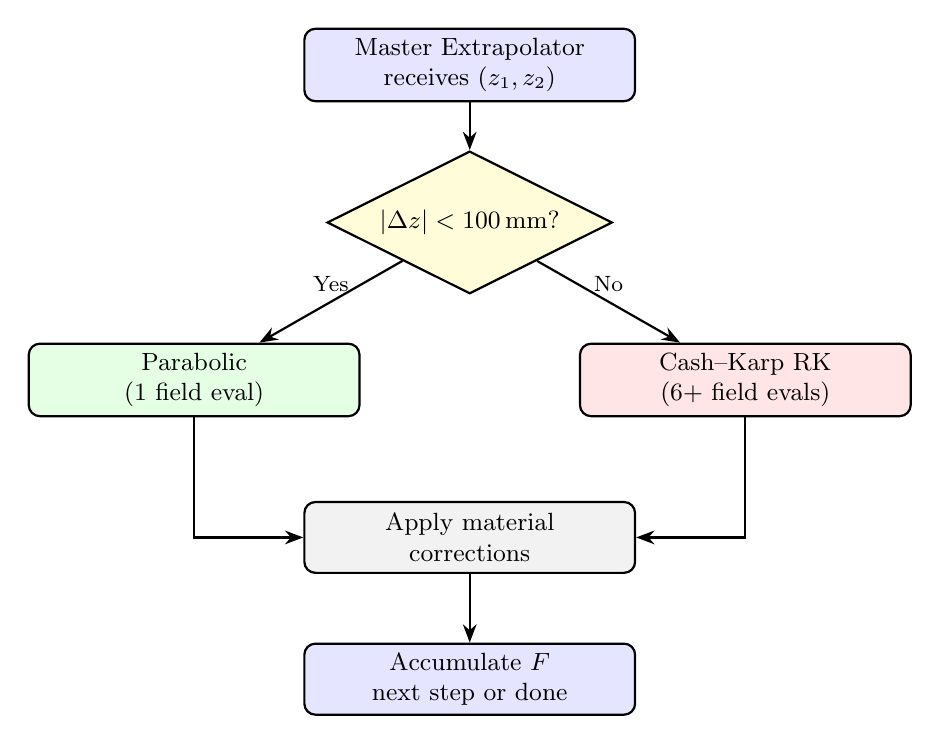
\begin{tikzpicture}[
  box/.style={draw, rounded corners, minimum width=4.2cm, minimum height=0.9cm,
              align=center, font=\small},
  decision/.style={draw, diamond, aspect=2, minimum width=2.5cm, align=center,
                   font=\small},
  >=Stealth, thick
]
  \node[box, fill=blue!10] (master) at (0,0) {Master Extrapolator\\receives $(z_1, z_2)$};
  \node[decision, fill=yellow!15] (check) at (0,-2) {$|\dz| < 100$\,mm?};
  \node[box, fill=green!10] (parab) at (-3.5,-4) {Parabolic\\(1 field eval)};
  \node[box, fill=red!10] (rk) at (3.5,-4) {Cash--Karp RK\\(6+ field evals)};
  \node[box, fill=gray!10] (mat) at (0,-6) {Apply material\\corrections};
  \node[box, fill=blue!10] (accum) at (0,-7.8) {Accumulate $F$\\next step or done};

  \draw[->] (master) -- (check);
  \draw[->] (check) -- node[above,font=\footnotesize]{Yes} (parab);
  \draw[->] (check) -- node[above,font=\footnotesize]{No} (rk);
  \draw[->] (parab) |- (mat);
  \draw[->] (rk) |- (mat);
  \draw[->] (mat) -- (accum);
\end{tikzpicture}
\caption{Master Extrapolator dispatch flow.}
\label{fig:master-flow}
\end{figure}


%=============================================================================
\section{QMTest Regression Testing Pipeline}\label{sec:qmtest}
%=============================================================================

The LHCb CI system uses QMTest to validate extrapolator correctness. The
pipeline is:

\begin{figure}[H]
\centering
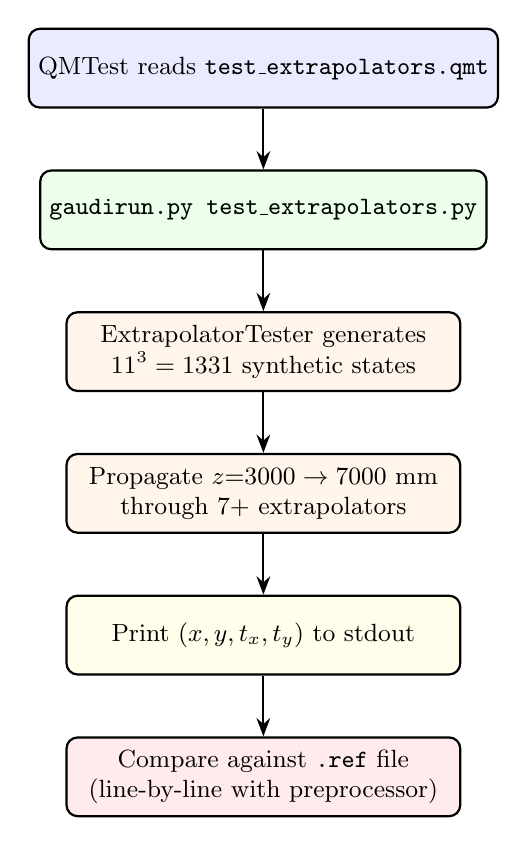
\begin{tikzpicture}[
  box/.style={draw, rounded corners, minimum width=5cm, minimum height=1cm,
              align=center, font=\small},
  >=Stealth, thick
]
  \node[box, fill=blue!8] (qmt) at (0,0)
    {QMTest reads \texttt{test\_extrapolators.qmt}};
  \node[box, fill=green!8] (gaudi) at (0,-1.8)
    {\texttt{gaudirun.py test\_extrapolators.py}};
  \node[box, fill=orange!8] (algo) at (0,-3.6)
    {ExtrapolatorTester generates\\$11^3 = 1331$ synthetic states};
  \node[box, fill=orange!8] (prop) at (0,-5.4)
    {Propagate $z{=}3000 \to 7000$~mm\\through 7+ extrapolators};
  \node[box, fill=yellow!8] (out) at (0,-7.2)
    {Print $(x,y,t_x,t_y)$ to stdout};
  \node[box, fill=red!8] (val) at (0,-9.0)
    {Compare against \texttt{.ref} file\\(line-by-line with preprocessor)};

  \draw[->] (qmt) -- (gaudi);
  \draw[->] (gaudi) -- (algo);
  \draw[->] (algo) -- (prop);
  \draw[->] (prop) -- (out);
  \draw[->] (out) -- (val);
\end{tikzpicture}
\caption{QMTest pipeline for extrapolator regression testing.}
\label{fig:qmtest-pipeline}
\end{figure}

\subsection{Test State Grid}

The \texttt{ExtrapolatorTester} algorithm generates a Cartesian grid of
initial track states:
\begin{itemize}[nosep]
  \item $q/p \in [-0.0004,\,+0.0004]~\text{MeV}^{-1}$ (momenta $\gtrsim 2.5$~GeV)
  \item $t_x \in [-0.3,\,+0.3]$, \quad $t_y \in [-0.25,\,+0.25]$
  \item 11~bins per dimension $\Rightarrow$ 1331 test states
  \item Initial position: $x = t_x \cdot z_\text{init}$,
        $y = t_y \cdot z_\text{init}$ (tracks from origin)
  \item Propagation: $z_\text{init} = 3000 \to z_\text{final} = 7000$~mm
\end{itemize}

\subsection{Extrapolators Under Test}

The CI test (\texttt{test\_extrapolators.py}) exercises:
\begin{enumerate}[nosep]
  \item Cash--Karp (Reference)
  \item Bogacki--Shampine~3(2)
  \item Verner~7(6)
  \item Verner~9(8)
  \item Tsitouras~5(4) (verbose mode)
  \item Kisel
  \item Herab
\end{enumerate}

\subsection{Validation}

The stdout output is compared line-by-line against a reference file
(\texttt{test\_extrapolators.ref}, 10\,778 lines).
A \texttt{LineSkipper} preprocessor strips non-deterministic lines
(timing, IOV, DD4Hep messages) before comparison.
The test passes if and only if all remaining lines match exactly.

Platform-specific reference files exist for different architectures
(e.g.\ \texttt{.ref.armv8}, \texttt{.ref.x86\_64\_v3\-opt})
to account for floating-point differences.


%=============================================================================
\section{SOA Benchmark Tester}\label{sec:soa}
%=============================================================================

For performance analysis (distinct from regression testing), the
\texttt{TrackExtrapolatorTesterSOA} writes ROOT NTuples with quantitative
data:

\begin{table}[H]
\centering
\caption{NTuple columns written by \texttt{TrackExtrapolatorTesterSOA}.}
\begin{tabular}{@{}p{5cm}ll@{}}
\toprule
\textbf{Column} & \textbf{Type} & \textbf{Description} \\
\midrule
\texttt{qop, x\_i, y\_i, tx\_i, ty\_i}
  & float & Input state \\
\texttt{x\_f, y\_f, tx\_f, ty\_f}
  & float & Reference output \\
\texttt{dx, dy, dtx, dty}
  & float & Residuals \\
\texttt{time}
  & float & Propagation time (ns) \\
\texttt{success}
  & int & StatusCode \\
\texttt{field\_cycles}, \ldots
  & int64 & RDTSC sub-timers \\
\texttt{nsteps, nrejected}
  & int & Adaptive step stats \\
\bottomrule
\end{tabular}
\end{table}


%=============================================================================
\section{Summary Table of Extrapolators}\label{sec:summary}
%=============================================================================

\begin{table}[H]
\centering
\caption{Complete inventory of LHCb track extrapolators.}
\footnotesize
\begin{tabular}{@{}lccl@{}}
\toprule
\textbf{Extrapolator} & \textbf{Field evals} & \textbf{Order} & \textbf{Use case} \\
\midrule
\texttt{TrackLinearExtrapolator}       & 0      & 1    & Field-free regions \\
\texttt{TrackParabolicExtrapolator}    & 1      & 2    & Short distances ($<100$\,mm) \\
\texttt{TrackRungeKuttaExtrapolator}   & 6/step & 5(4) & General, production default \\
\texttt{TrackSTEPExtrapolator}         & 2/step & 4    & ATLAS-style RKN \\
\texttt{TrackHerabExtrapolator}        & 6/step & 5(4) & HERA-B legacy \\
\texttt{TrackKiselExtrapolator}        & 3      & 1--3 & CBM Taylor expansion \\
\texttt{TrackParametrizedExtrapolator} & 0$^*$  & poly & Plane-to-plane shortcuts \\
\texttt{TrackMasterExtrapolator}       & ---    & ---  & Dispatcher + material \\
\bottomrule
\end{tabular}
\begin{flushleft}
\footnotesize $^*$Pre-trained at initialisation using RK.
\end{flushleft}
\end{table}


\end{document}
